%% Direttive TeXworks:
% !TeX root = ../maltoni_niccolo_tesi.tex
% !TEX encoding = UTF-8 Unicode
% !TEX program = arara
% !TEX TS-program = arara
% !TeX spellcheck = it-IT

%% Direttive Arara:
% arara: pdflatex: { shell: yes, synctex: yes, action: batchmode, options: "-halt-on-error -file-line-error-style" }
% arara: frontespizio
% arara: biber
% arara: pdflatex: { shell: yes, synctex: yes, action: batchmode, options: "-halt-on-error -file-line-error-style" }
% arara: pdflatex: { shell: yes, synctex: yes, action: nonstopmode, options: "-halt-on-error -file-line-error-style" }

\appendix
\chapter{L'interfaccia \texttt{Effect}}\label{appendix:effect}
    % \begin{minted}{java}
    % \begin{minipage}{\linewidth}
    \begin{lstlisting}[language=Java]
        public interface Effect extends Serializable {
            /**
             * Applies the effect.
             *
             * @param graphic
             *            Graphics2D to use
             * @param node
             *            the node to draw
             * @param x
             *            x screen position
             * @param y
             *            y screen position
             */
            void apply(Graphics2D graphic, Node<?> node, int x, int y);

            /**
             * @return a color which resembles the color of this effect
             */
            Color getColorSummary();

            @Override // Should override hashCode() method
            int hashCode();

            @Override // Should override equals() method
            boolean equals(Object obj);
        }
    \end{lstlisting}
    % \end{minipage}
    % \end{minted}

\chapter{L'interfaccia \texttt{EffectFX}}\label{appendix:effectfx}
    % \begin{minted}{java}
    % \begin{minipage}{\linewidth}
    \begin{lstlisting}[language=Java]
        /**
         * Graphical visualization of something happening in the environment.
         */
        public interface EffectFX extends Serializable {

            /**
             * Computes a queue of commands to Draw something.
             *
             * @param environment the environment to gather data from
             * @param <T>         the {@link Concentration} type
             * @return the queue of commands that should be run to draw the effect
             */
            <T> Queue<DrawCommand> computeDrawCommands(Environment<T> environment);

            /**
             * Gets the name of the effect.
             *
             * @return the name of the effect
             */
            String getName();

            /**
             * Sets the name of the effect.
             *
             * @param name the name of the effect to set
             */
            void setName(String name);

            /**
             * Gets the visibility of the effect.
             *
             * @return the visibility of the effect
             */
            boolean isVisible();

            /**
             * Sets the visibility of the effect.
             *
             * @param visibility the visibility of the effect to set
             */
            void setVisibility(boolean visibility);
        }
    \end{lstlisting}
    % \end{minipage}
    % \end{minted}

    \chapter{L'interfaccia \texttt{EffectGroup}}\label{appendix:effectgroup}
        % \begin{minted}{java}
        % \begin{minipage}{\linewidth}
        \begin{lstlisting}[language=Java]
            /**
             * Models a group of effects. Each effect has a different priority of
             * visualization.
             */
            public interface EffectGroup extends Serializable, Queue<EffectFX> {

                /**
                 * Computes all the commands for all the visible effects in this group.
                 *
                 * @param environment the environment to gather data from
                 * @param <T>         the {@link Concentration} type
                 * @return the queue of commands that should be run to draw the effects of the group
                 * @see EffectFX#computeDrawCommands(Environment)
                 */
                <T> Queue<DrawCommand> computeDrawCommands(Environment<T> environment);

                /**
                 * Gets the name of the group.
                 *
                 * @return the name of the group
                 */
                String getName();

                /**
                 * Sets the name of the group.
                 *
                 * @param name the name of the group
                 */
                void setName(String name);

                /**
                 * Checks if an effect is present in the group.
                 *
                 * @param effect the effect to search
                 * @return the position, or -1 if not present
                 */
                int search(EffectFX effect);

                /**
                 * Returns the visibility of the group.
                 *
                 * @return the visibility
                 */
                boolean isVisible();

                /**
                 * Sets the visibility of the group.
                 *
                 * @param visibility the visibility
                 */
                void setVisibility(boolean visibility);

                /**
                 * Returns the visibility of the specified effect.
                 *
                 * @param effect the effect
                 * @return the visibility
                 * @throws IllegalArgumentException if can't find the effect
                 * @see EffectFX#isVisible()
                 */
                boolean getVisibilityOf(EffectFX effect);

                /**
                 * Sets the visibility of the specified effect.
                 *
                 * @param effect     the effect
                 * @param visibility the visibility to set
                 * @throws IllegalArgumentException if can't find the effect
                 * @see EffectFX#setVisibility(boolean)
                 */
                void setVisibilityOf(EffectFX effect, boolean visibility);

                /**
                 * Changes the specified offset priority of the specified offset.
                 *
                 * @param effect the effect
                 * @param offset the offset; it can be positive or negative
                 * @throws IllegalArgumentException if can't find the effect
                 */
                void changePriority(EffectFX effect, int offset);

                /* Is suggested to override Object default equals method. */
                @Override
                int hashCode();

                /**
                 * Compares the {@link EffectGroup EffectGroup}s. The result is true if and
                 * only if the argument is not {@code null} and every {@link EffectFX}
                 * contained is not {@code null} and {@link EffectFX#equals(Object) equal} to
                 * the corresponding in the comparing {@code EffectGroup} (order is
                 * important!) and the group has the same name, visibility and transparency.
                 *
                 * @see Object#equals(Object)
                 */
                /* Is suggested to override Object default equals method. */
                @Override
                boolean equals(Object obj);
            }
        \end{lstlisting}
        % \end{minipage}
        % \end{minted}

\chapter{Implementazioni di \texttt{EffectFX} e Proprietà serializzabili}\label{appendix:effectsAndProps}
    \begin{figure}[htbp]
      \centering
      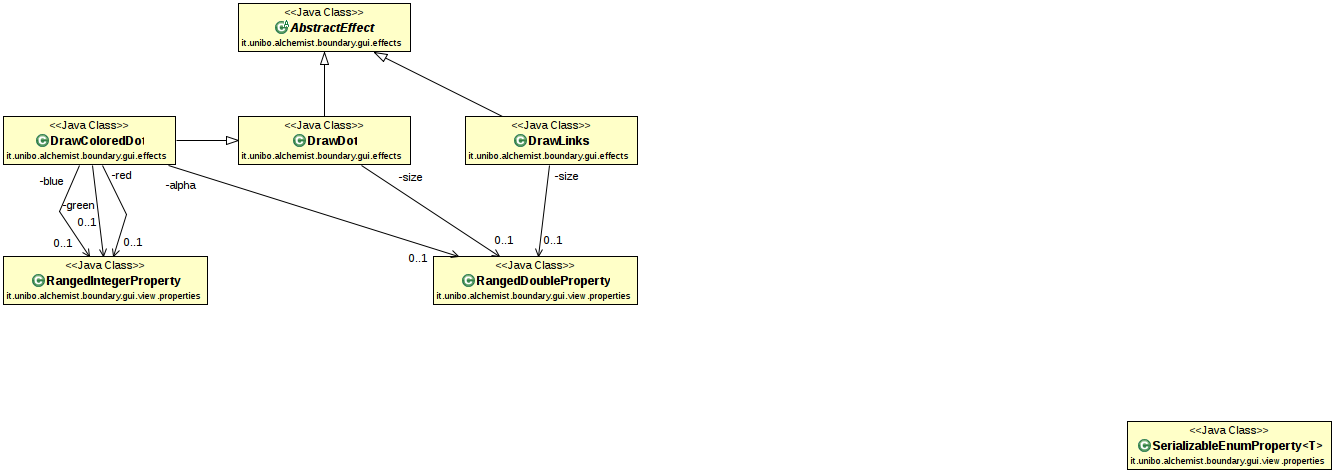
\includegraphics[scale=0.7]{img/EffectAndPropertiesUML}
      \caption{Il diagramma UML delle classi mostra le relazioni tra gli effetti implementati e le proprietà custom utilizzate}
    \end{figure}
